\chapter{Circuiti RC e RL (C3)}

\section{Corrente impulsata}
\subsubsection{Introduzione}

\subsection{Procedimento}

Oggetto di studio di questa esperienza è l'andamento della differenza di potenziale ai capi di resistenza e capacità o induttanza.
A tal fine costruiamo un circuito con i seguenti elementi:
[disegno]

\begin{itemize}
  \item Generatore di onde
  \item Un condensatore di capacità 367 nF più errore
  \item Un'induttore di induttanza sconosciuta
  \item Un oscilloscopio con due sonde
  \item Una resistenza di 667 Ohm (più errore)
\end{itemize}

Per simulare l'apertura e la chiusura del circuito impostiamo nel generatore la modalità onda quadra. Una sonda posta prima del condensatore mostra sullo schermo dell'oscilloscopio il segnale.  
Una seconda sonda, posta ai capi della resistenza, visualizza la forma dell'onda caratteristica della carica o della scarica di un condensatore.

Raccogliamo i dati (differenza di potenziale e tempo) dall'onda visualizzata sul display dell'oscilloscopio, tramite i cursori. Interpoliamo i dati raccolti con la curva caratteristica della carica/scarica di un condensatore.

Il valore stimato dall'interpolazione è $\tau=RC$ dell'equazione
$$V_R = \varepsilon e^{-t/\tau}$$

\subsection{Dati}
\subsubsection{Circuito RC}

\subsubsection{Circuito RL}

\subsection{Analisi}

\subsubsection{Circuito RC}
\subsubsection{Circuito RL}
\subsection{Analisi delle incertezze}


\section{Corrente alternata}
\subsection{Procedimento}
\subsection{Raccolta dati}
\subsubsection{Circuito RC}
\begin{center}
 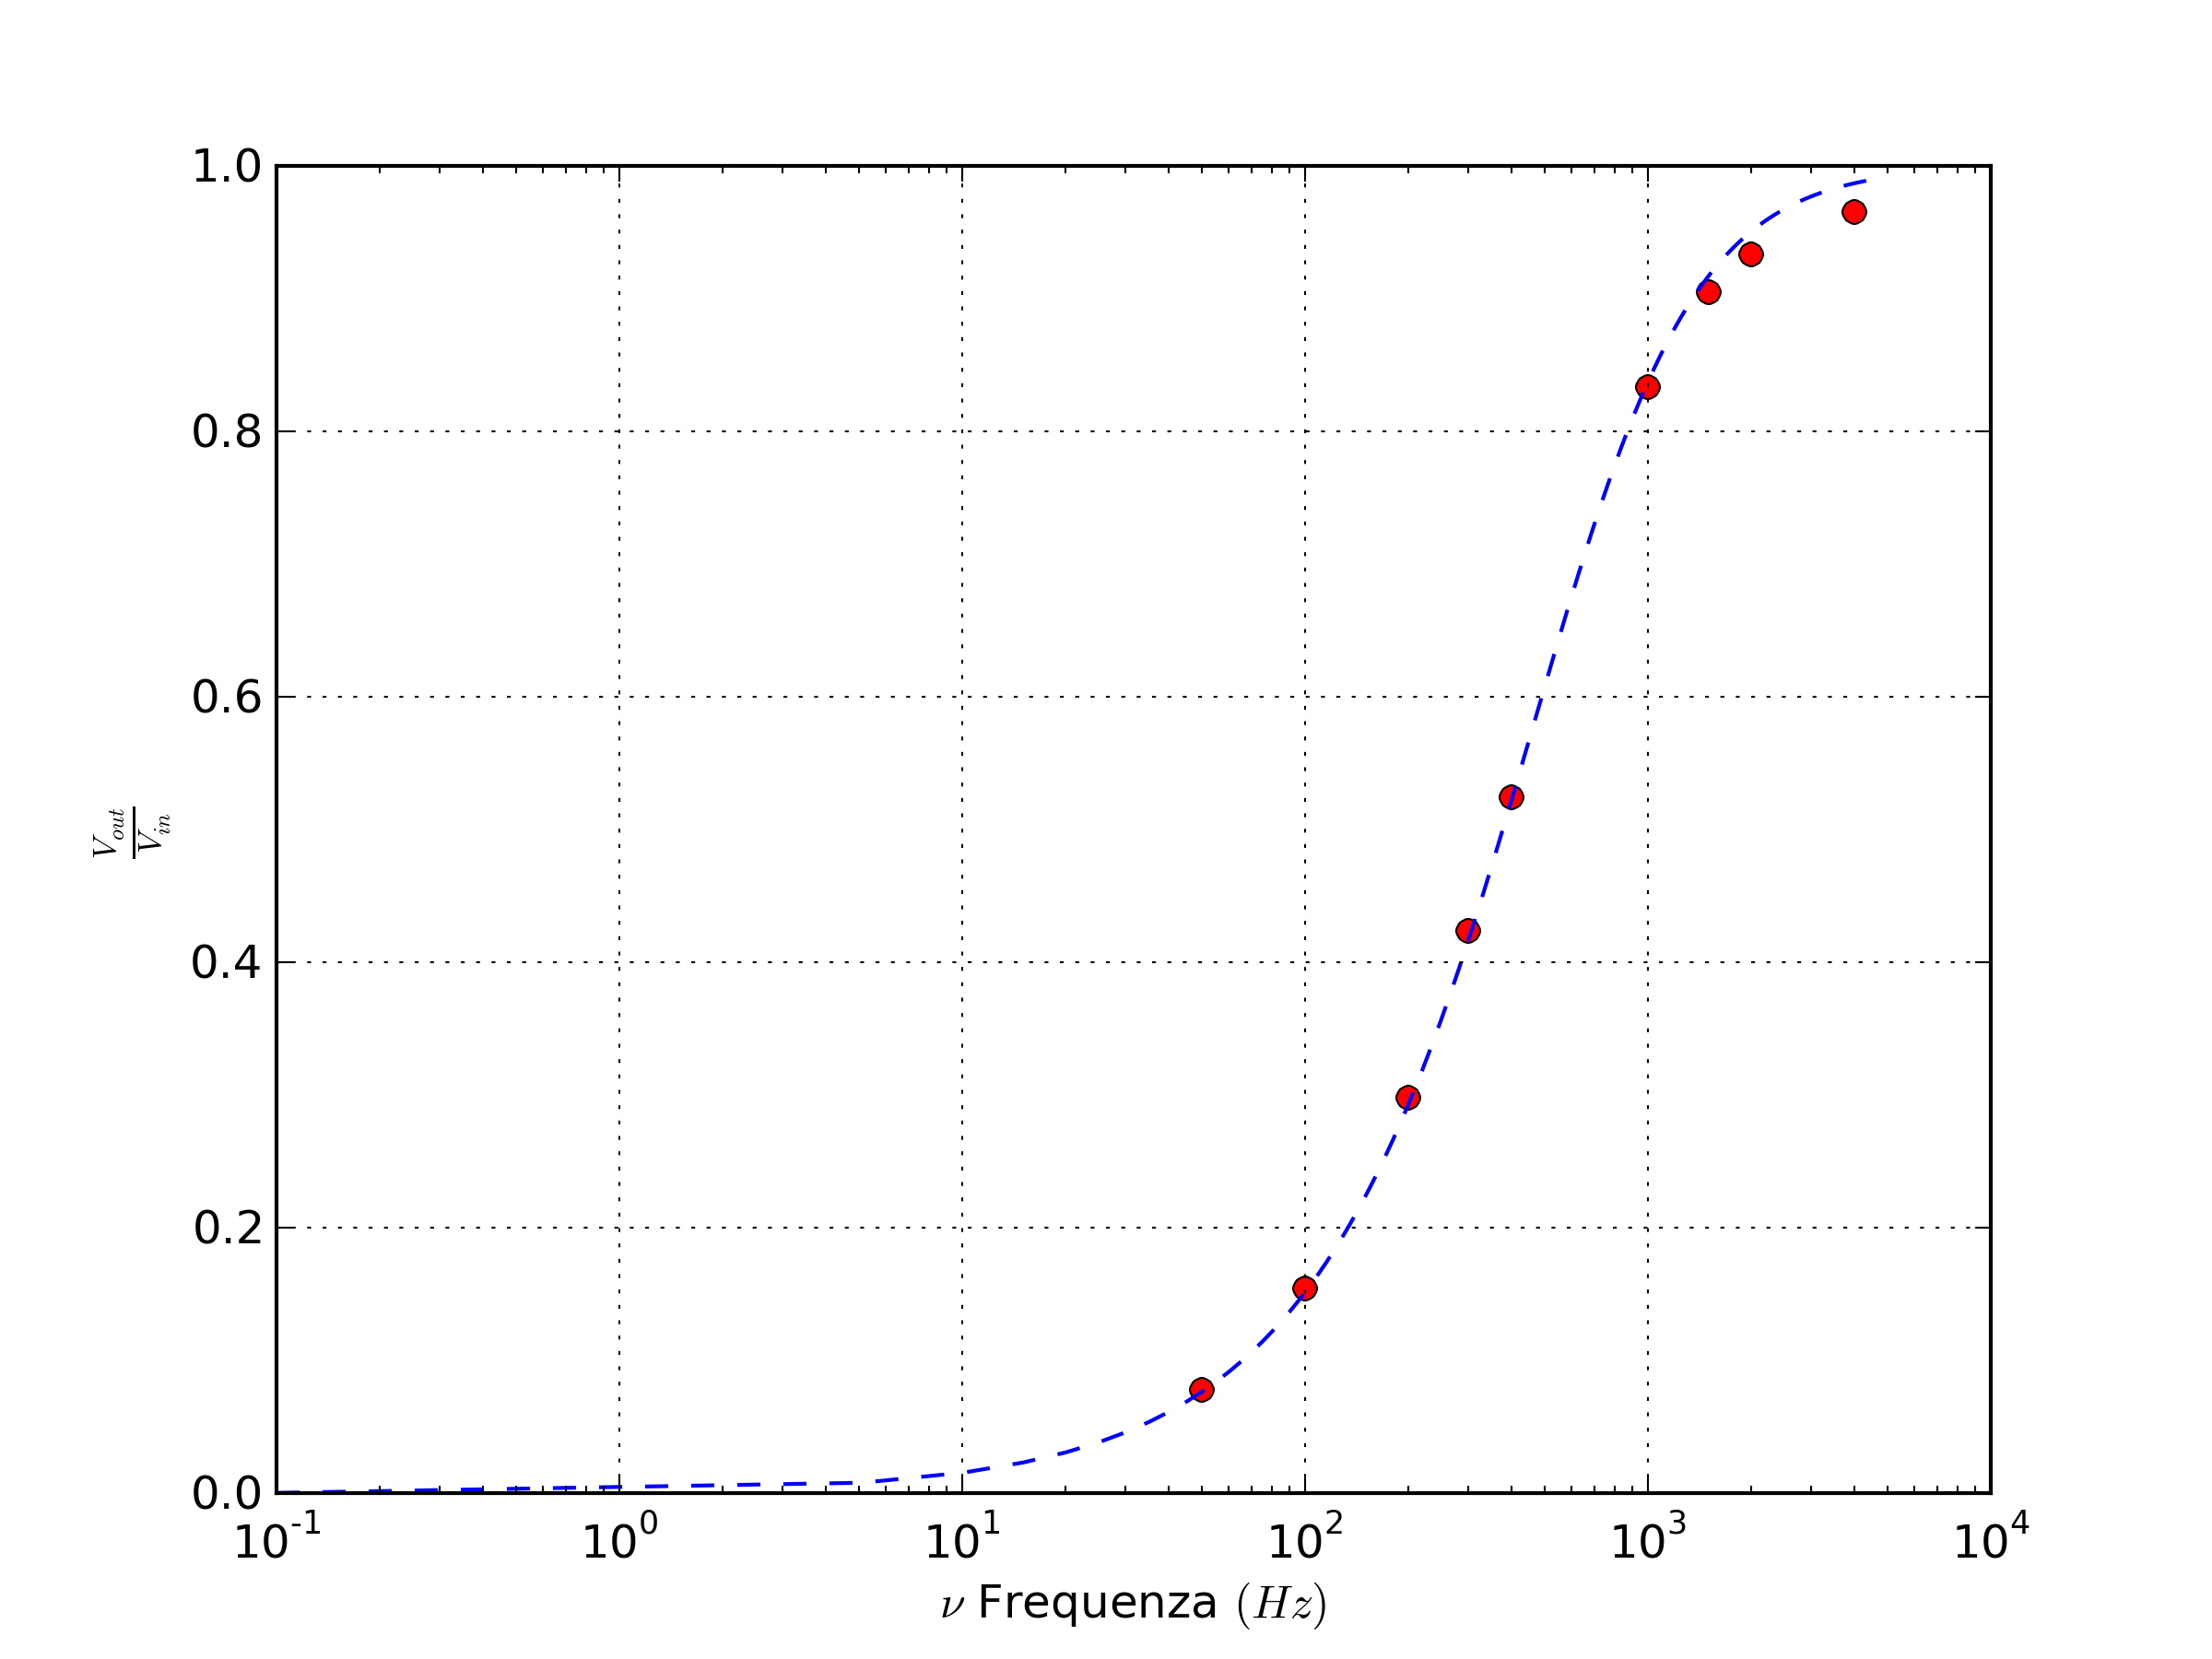
\includegraphics[scale=0.50]{grafici/C3/ddpcond.png}
\end{center}
\subsubsection{Circuito RL}
\begin{center}
 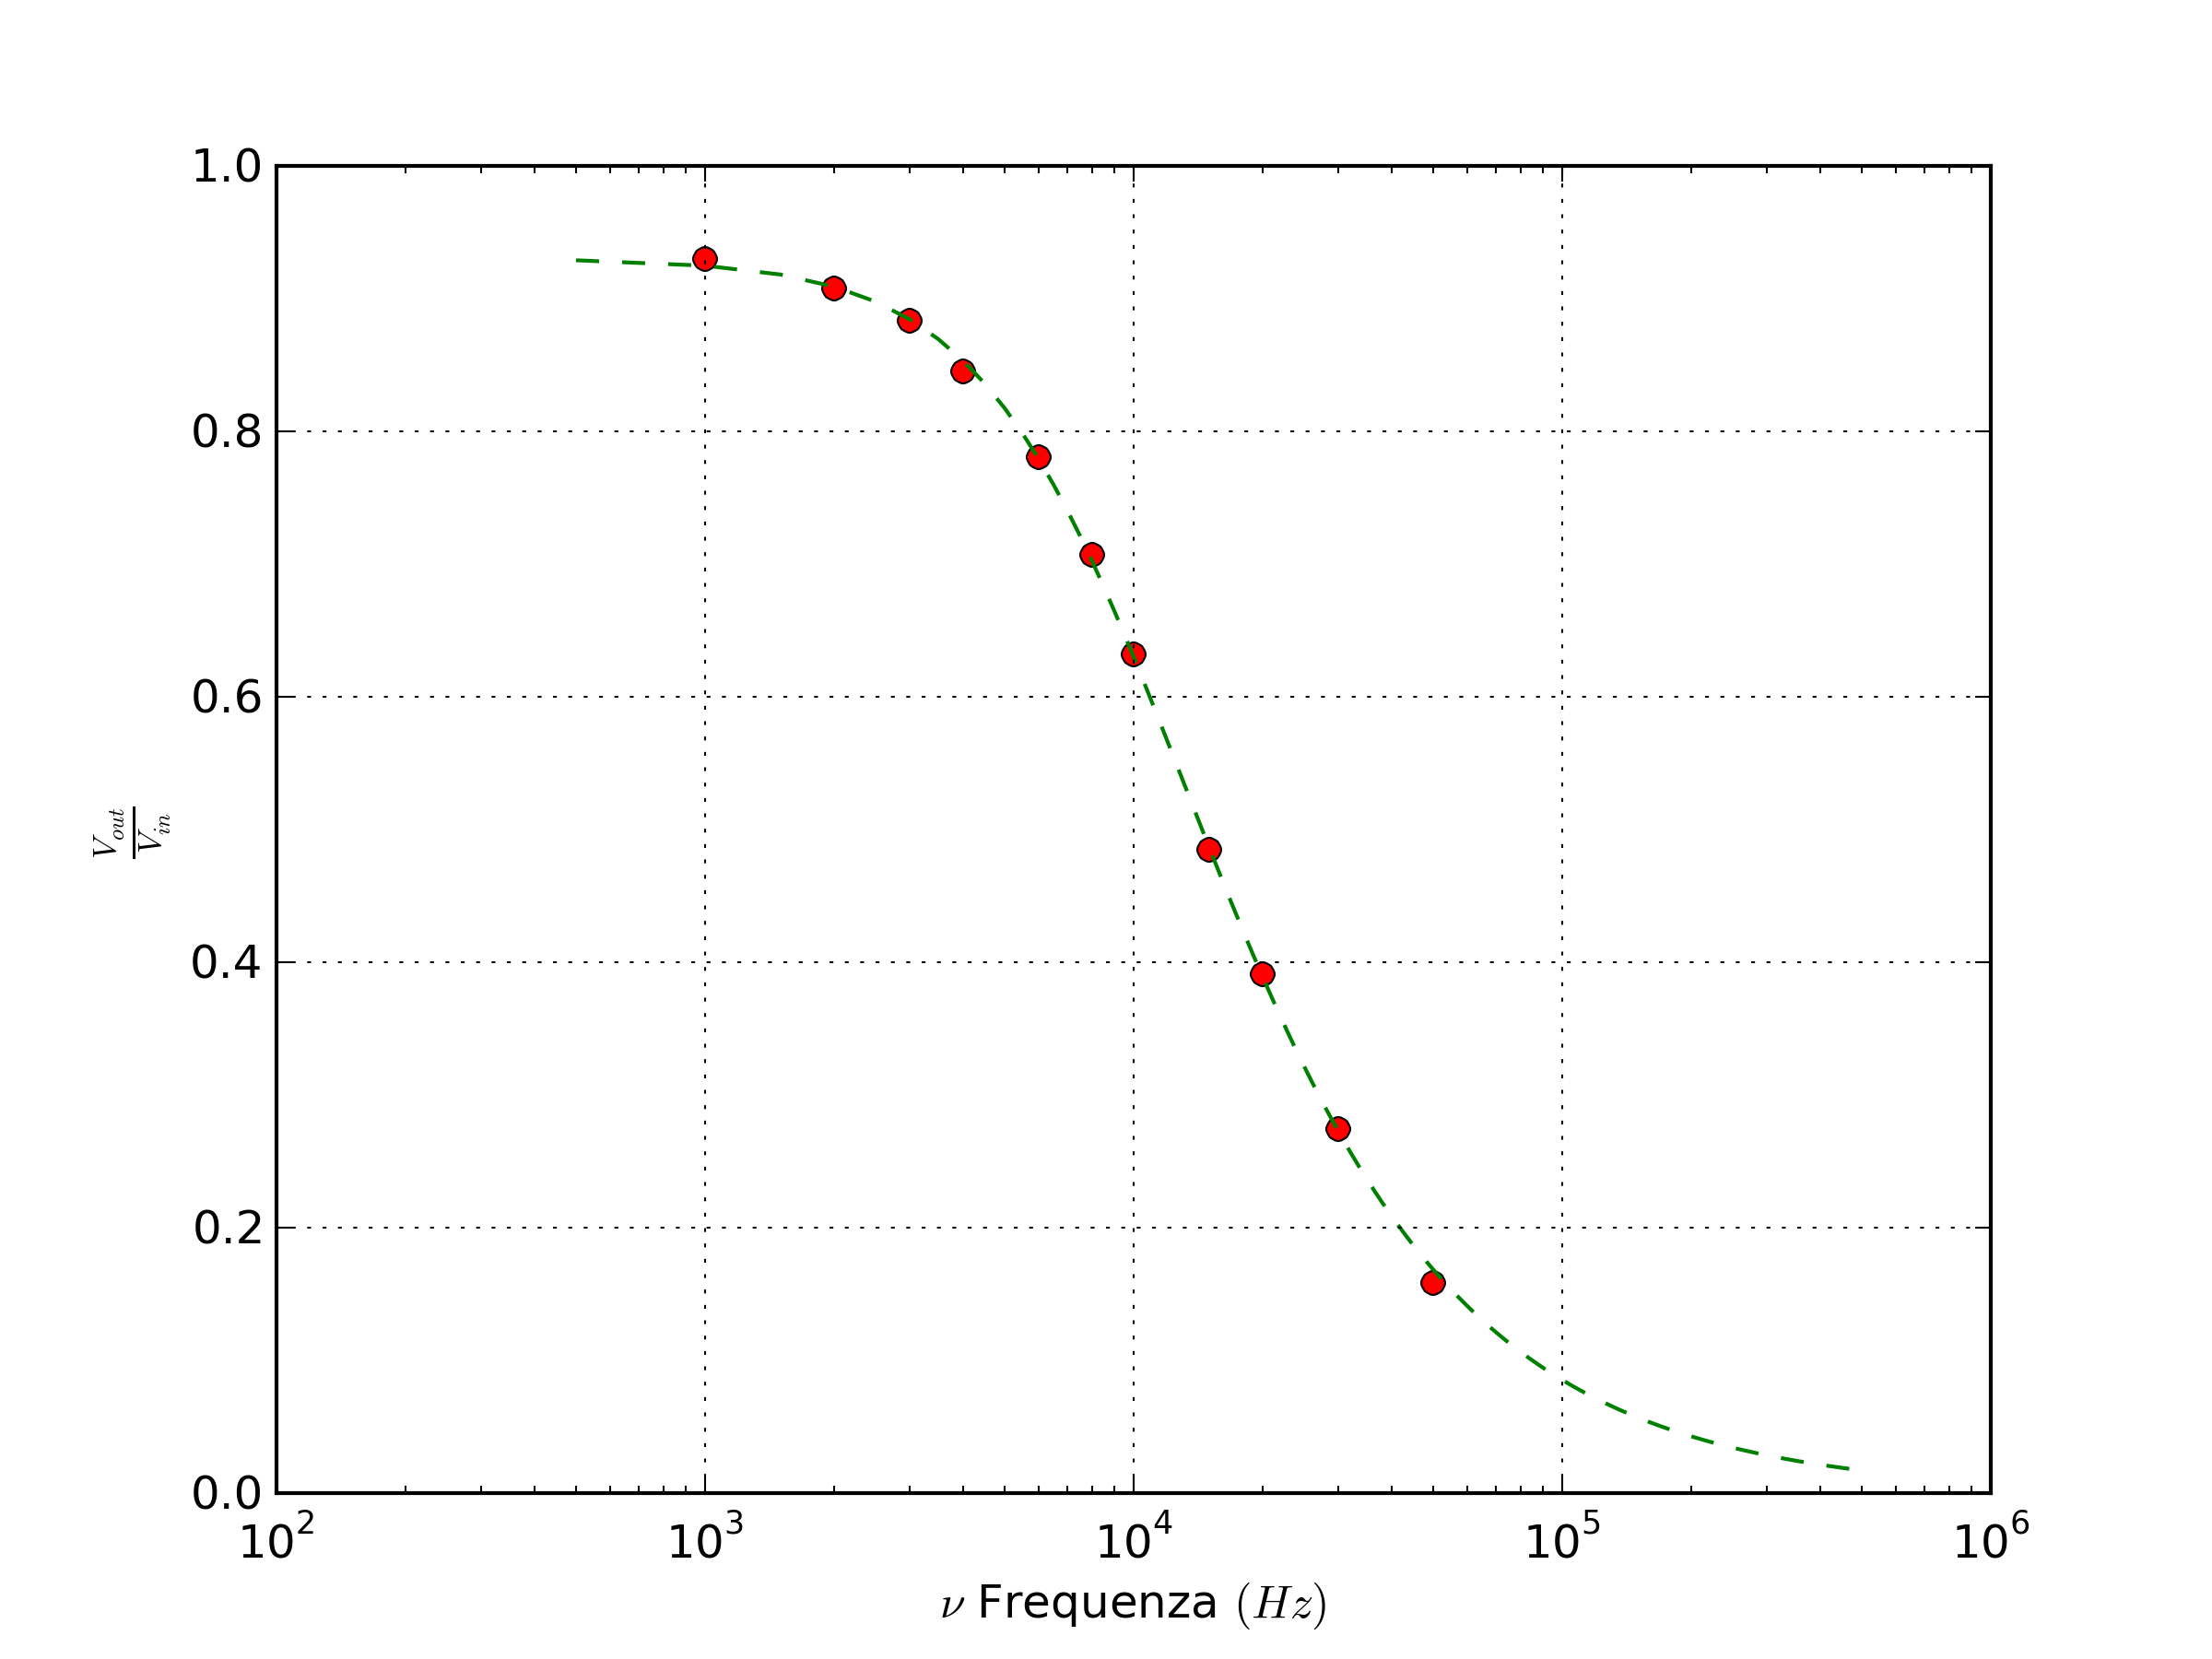
\includegraphics[scale=0.50]{grafici/C3/ddpindu.png}
\end{center}
\section{Conclusioni}
\subsubsection{Circuito RC}
\subsubsection{Circuito RL}
